%%%%%%%%%%%%%%%%%%%%%%%%%%%%%%%%%%%%%%%%%%%%%%%%%%%%%%%%%%%%%%%%%%%%%%%%%%%%%%%%
%2345678901234567890123456789012345678901234567890123456789012345678901234567890
%        1         2         3         4         5         6         7         8


\documentclass[a4paper, 10pt, conference] {article}        
                                                           

%\IEEEoverridecommandlockouts                              % This command is only
                                                          % needed if you want to
                                                          % use the \thanks command
%\overrideIEEEmargins
% See the \addtolength command later in the file to balance the column lengths
% on the last page of the document



% The following packages can be found on http:\\www.ctan.org
\usepackage{graphicx} % for pdf, bitmapped graphics files
\usepackage{caption}
\usepackage{float}
\usepackage{subcaption}
\usepackage{epsfig} % for postscript graphics files
\usepackage{mathptmx} % assumes new font selection scheme installed
\usepackage{times} % assumes new font selection scheme installed
\usepackage{amsmath} % assumes amsmath package installed
\usepackage{amssymb}  % assumes amsmath package installed
\usepackage[margin=1.5cm]{geometry}
\usepackage{mathtools}
%\usepackage{enumerate}
\usepackage{enumitem}
\usepackage{lipsum}
\usepackage{mcode} %  [framed]
\begin{document}
\date{}
\title{\LARGE \bf
B31SE2 – Matlab Lab 2
Fourier Theory. Image compression/quantization
}

\author{ \parbox{5 in}{\centering Daniel Barmaimon \\
%         \thanks{*Use the $\backslash$thanks command to put information here}\\
         \ Advanced Image Analysis - Vibot Master Degree\\
         \ Heriot Watt University\\         
}}

\maketitle
%\thispagestyle{empty}
%\pagestyle{empty}


\section{Introduction}
The size of the images captures nowadays by cameras is increasing as much as the development of the hardware. For avoiding the problem of the size for storing them and reduce the time for transferring techniques for compress the images are commonly used. In this lab some of this techniques will be studied and analyzed. The quality of quantized and compressed images is going to be compared with the original images.
\section{Implementation of Haar Wavelet Transform and Inverse Haar Wavelet Transform}
The reduction compression of the image could be implemented by using some linear combinations over the original image. The use of this matrix is based in dividing the image in low frequencies (approximation level) that will be obtained by the average of two consecutive elements of a signal, and the high frequencies (detail level) that will be obtained by the gradient between two consecutive elements of a signal. This step could be repeated iteratively until reach the level of compression desired. 
The matrix W, for applying over a signal of size N, where N in this case is 8, is the following.
\begin{figure}[H]
	\centering
	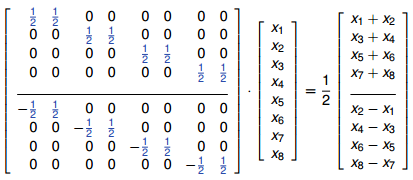
\includegraphics[width=0.5\textwidth]{reportImages/W.png} %
	\caption{Discrete Haar Wavelet Transformation, $W_{8}$}
	\label{W}
\end{figure}

In the same way, it is possible to apply the inverse of this transformation, what is quite easy to calculate because $W_{N}^{-1} = W_{N}^{T}$
The previous theory was applicable over a signal of one dimension. To apply it over an image it will be necessary to apply one transformation for each of the dimensions. This will lead Eq.\ref{B}.
 \begin{equation}
 B = W_{M}AW_{N}^{T}
 \label{B}
 \end{equation}
 The code implemented to get the Haar Wavelet transformation, its inverse, and computation of the matrices needed for its generation are shown below.
 
 \begin{lstlisting}
					 function [ imOut ] = HaarTransform( im, iter )
					 [n,m] = size(im);
					 [Wn,Wm] = generateMatrices( n,m );
					 % Get the output image for the first iteration
					 B=Wn*double(im)*Wm'; 
					 imOut = B; 
					 % Check if is the last iteration
					 if (iter == 1), return; end;    
					 % Recursively get the image
					 imOut(1:n/2,1:m/2) = HaarTransform(imOut(1:n/2,1:m/2), iter-1); 
					 end
					 
					 
					 
					 
					 function [ imOut ] = inverseHaarTransform( im, iter )
					 [n,m] = size(im);
					 % Get the output image for the first iteration
					 imOut = im;
					 % Check if all iterations have been performed
					 if (iter == 0), return; end; 
					 imOut(1:n/2,1:m/2) = inverseHaarTransform(imOut(1:n/2,1:m/2), iter-1);
					 % Update the matrices after getting the Inverse Wavelet Tranform   
					 [Wn,Wm] = generateMatrices( n,m );
					 imOut = Wn'*double(imOut)*Wm;
					 end
					 
					 function [ Wn, Wm ] = generateMatrices( n, m )
					 H = zeros(n/2,n);
					 G = zeros(n/2,n);
					 % Repeating the each column to generate H, G
					 combos = eye(n/2); 
					 for i =0:size(combos,1)-1
					 H(:,2*i+1) = 1/sqrt(2)*combos(:,i+1);   
					 H(:,2*(i+1)) = H(:,2*i+1);
					 G(:,2*i+1) = -H(:,2*i+1);  
					 G(:,2*(i+1))= H(:,2*i+1);
					 end
					 Wn = double([H;G]);
					 % Repeating the process for dimension m
					 H = zeros(m/2,m);
					 G = zeros(m/2,m);
					 combos = eye(m/2); 
					 for i =0:size(combos,1)-1
					 H(:,2*i+1) = 1/sqrt(2)*combos(:,i+1); 
					 H(:,2*(i+1)) = H(:,2*i+1);
					 G(:,2*i+1) = -H(:,2*i+1);  
					 G(:,2*(i+1))= H(:,2*i+1);
					 end
					 Wm = double([H;G]);
					 end
		 
 \end{lstlisting}
 
 The result of applying consecutively this transformation over an image could be seen in Fig.\ref{Wavelet}
 \begin{figure}[H]
 	\centering
 	\begin{subfigure}{0.32\textwidth} 
 		\centering						
 		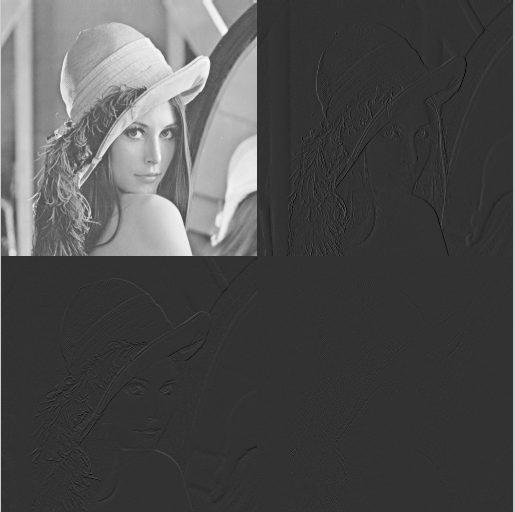
\includegraphics[scale=0.35]{reportImages/HaarW1.PNG}
 		\caption{Iteration = 1}
 	\end{subfigure}
 	\begin{subfigure}{0.32\textwidth}
 		\centering
 		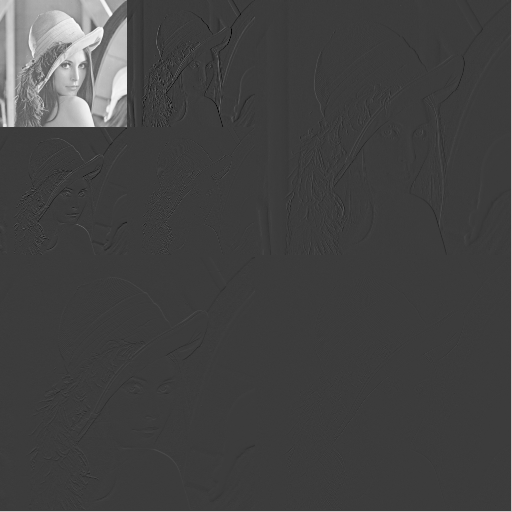
\includegraphics[scale=0.35]{reportImages/HaarW2.PNG}
 		\caption{Iteration = 2}
 	\end{subfigure}
 	
 	\caption{Wavelet transformation }
 	\label{Wavelet}
 \end{figure}
 It could be seen as pyramid, where the size is decrease to the half after each iteration. In the upper left corner is set the original image with it new size (averaged image). Next to it, to the right is located the horizontal gradient. Below the original image is located the vertical gradient. In the lower right corner is set the diagonal gradient vertical gradient (detailed images). \\
 
 In absence of noise during the compression, the original image can be obtained applying the inverse transformation the same number of iteration that the first one was used.\\
 
 In terms of implementation, calculation of the matrices H and G to create the matrix W are generated given the size of the original image, the posterior compression and decompression are implemented as recursive function with only two parameters, the image to compress (decompress) and the number of iterations.
 
 \section{Image Compression using DCT and Haar/Daubechies Wavelets}
 In this section the performance of DCT and Haar/Daubechies wavelets are going to be compared, using as metrics the MSE (minimum squared error) and PSNR (peak signal to noise ratio). In the first case the performance will be compared using the variation of the number of levels for the quantization to check the evolution of the methods.
 The second experiment will consist in the comparison between Daubechies with different vanishing moments.
 
 \subsection{Compression between DCT and Haar varying the number of quantization levels}
 The image of Lena will be compressed using the Discrete Cosine Transform (DCT) and the Haar Transform Wavelet (DWT), and both images will be quantized with the same number of levels for such quantization. The results could be observed quantitatively in Fig. and qualitatively after quantization and decompression in Fig.\ref{Levels}. 
 \begin{figure}[H]
 	\centering
 	\begin{subfigure}{0.49\textwidth} 
 		\centering						
 		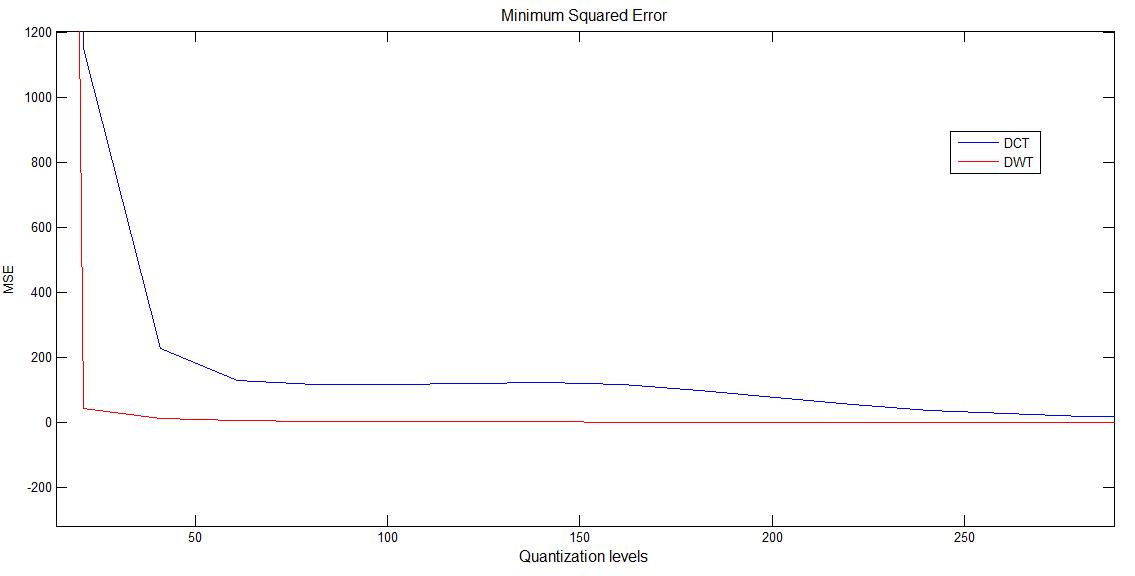
\includegraphics[scale=0.3]{reportImages/MSE.PNG}
 		\caption{Minimum Squared Error}
 	\end{subfigure}
 	\begin{subfigure}{0.49\textwidth}
 		\centering
 		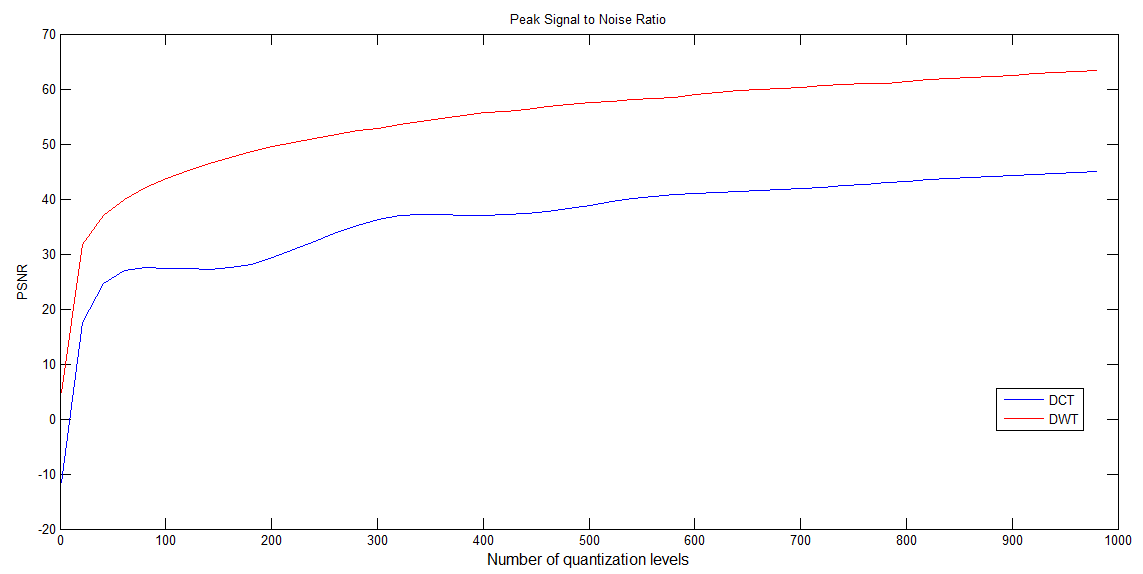
\includegraphics[scale=0.3]{reportImages/PSNR.PNG}
 		\caption{Peak Signal to Noise Ratio}
 	\end{subfigure}
	\caption{Metrics to compare the methods }
 	\label{Metrics1}
 \end{figure}
 
 \begin{figure}[H]
 	\centering
 	\begin{subfigure}{1\textwidth} 
 		\centering						
 		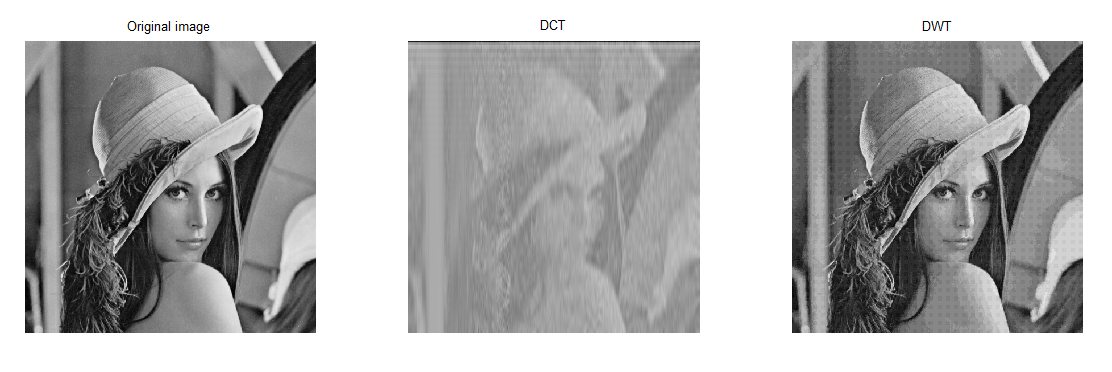
\includegraphics[scale=0.35]{reportImages/comparison_level21.PNG}
 		\caption{Number of levels = 21}
 	\end{subfigure}
 	\begin{subfigure}{1\textwidth}
 		\centering
 		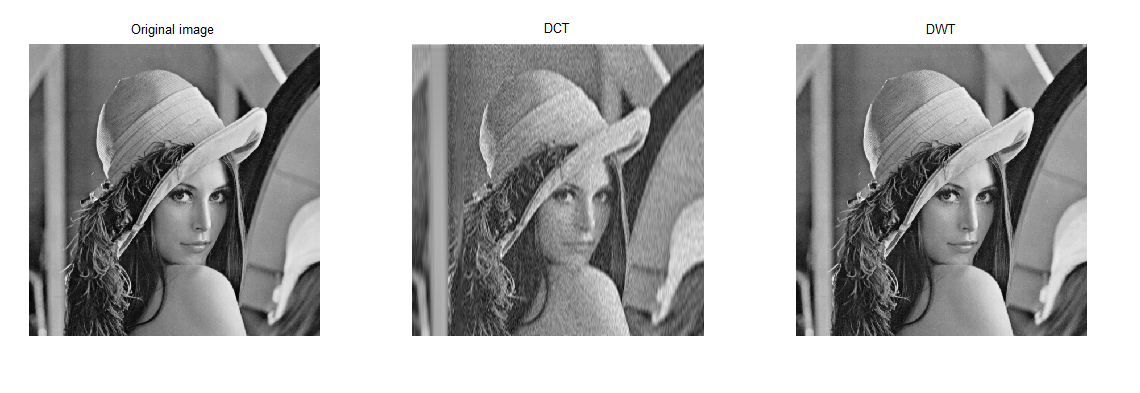
\includegraphics[scale=0.35]{reportImages/comparison_level61.PNG}
 		\caption{Number of levels = 61}
 	\end{subfigure}
 	\begin{subfigure}{1\textwidth}
 		\centering
 		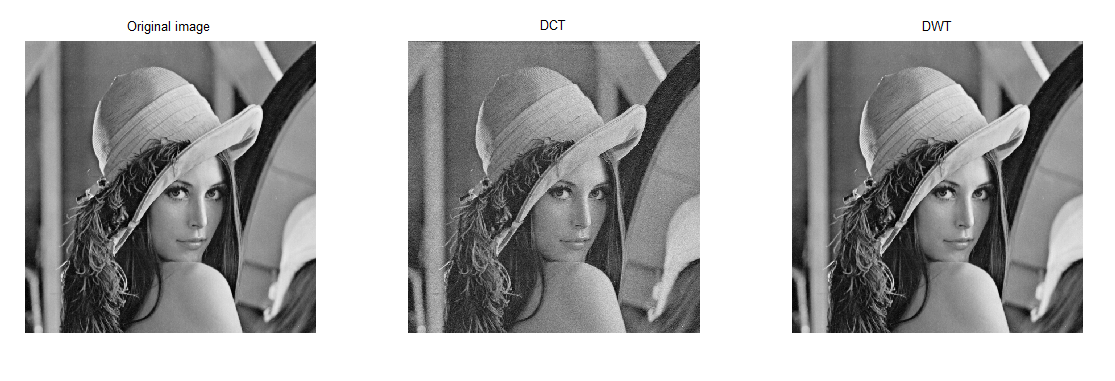
\includegraphics[scale=0.35]{reportImages/comparison_level201.PNG}
 		\caption{Number of levels = 201}
 	\end{subfigure}
 	
 	\caption{Comparison for different number of quantization levels }
 	\label{Levels}
\end{figure}
As result it should be said that the performance of the two methods are really close for a great number of quantization levels, but the smaller is this parameter the better is the DWT with respect to DCT to compress the image and quantize the image.
 
 
 \subsection{Comparison of Daubechies with different vanishing moments}
 In this section different levels of quantization will be applied with Daubechies wavelets with different vanishing moments. As it could be seen in the results, the higher is the number for the vanishing moment, the lower is the MSE and the higher is the PSNR (for high levels of quantization). For low amount of levels the best performance is given by D8 among the rest of the wavelets.
 \begin{figure}[H]
 	\centering
 	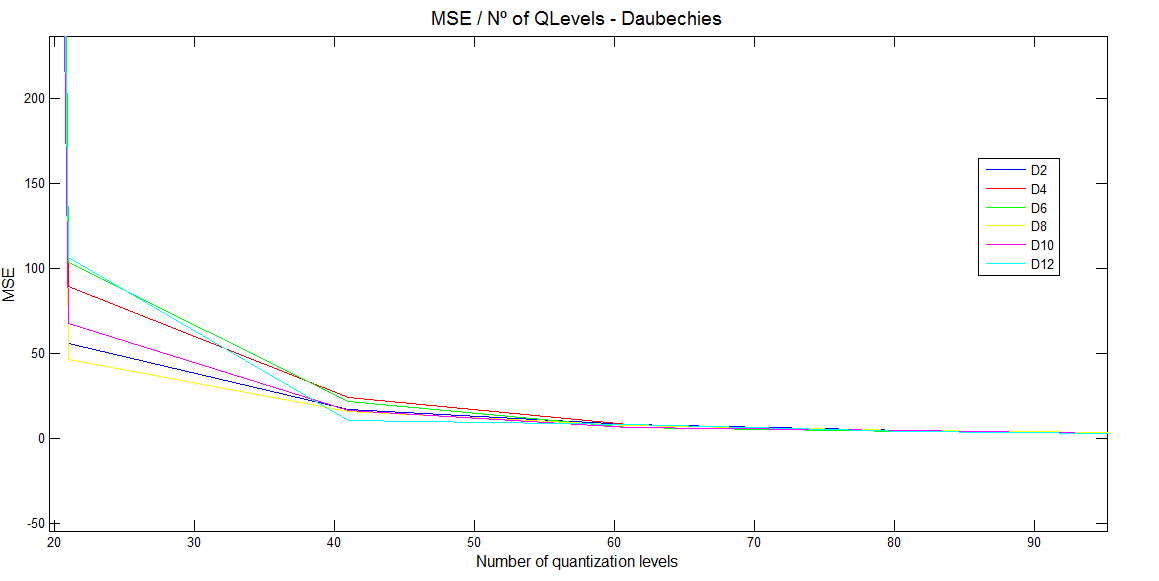
\includegraphics[scale=0.35]{reportImages/MSE_Daubechies.PNG}
 	\caption{Minimum Squared Error for Daubechies}
 	\label{MSEd}
 \end{figure}
 \begin{figure}[H]
 	\centering
 	\begin{subfigure}{1\textwidth}
 		\centering
 		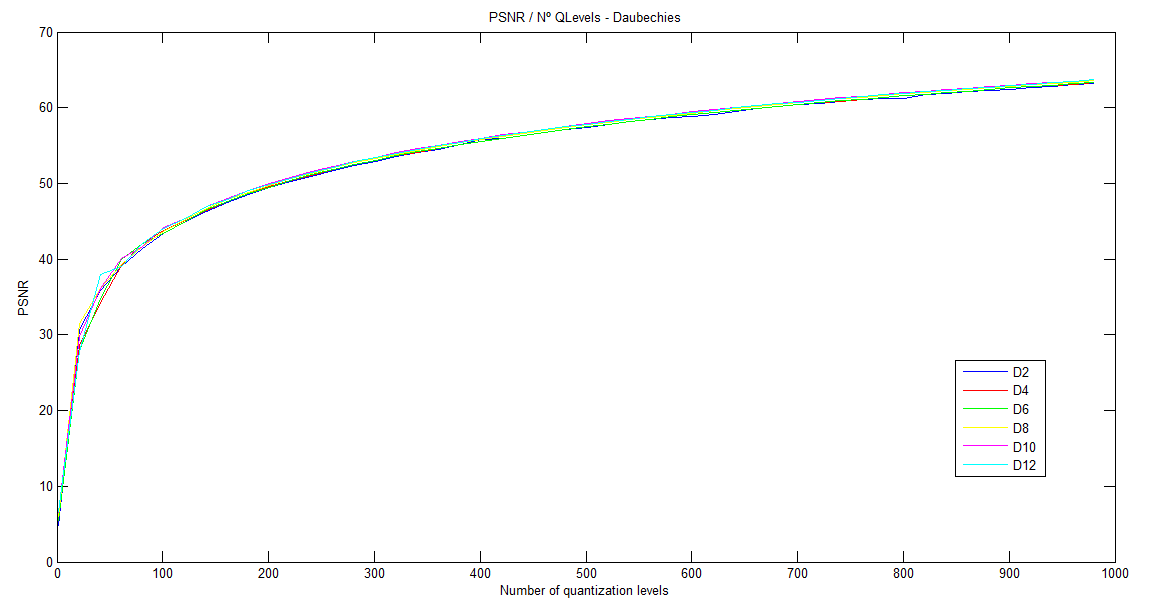
\includegraphics[scale=0.35]{reportImages/PSNR_Daubechies.PNG}
 		\caption{Peak Signal to Noise Ratio in dB}
 	\end{subfigure}
 	\begin{subfigure}{0.49\textwidth}
 		\centering
 		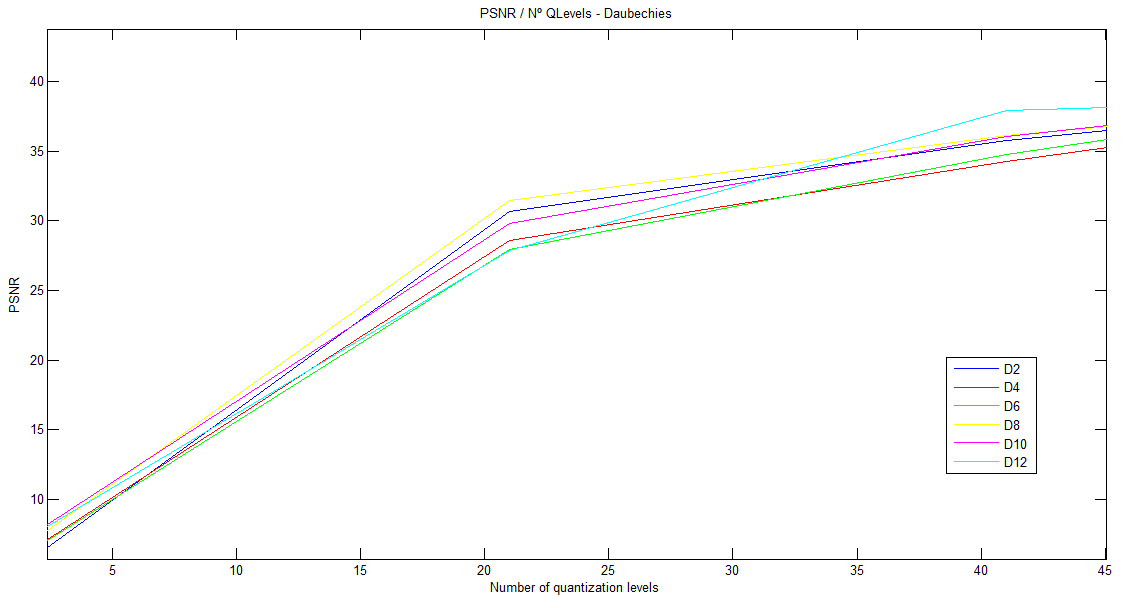
\includegraphics[scale=0.30]{reportImages/PSNR_Daubechies_detail.PNG}
 		\caption{Detail 1 of PSNR}
 	\end{subfigure}
 	\begin{subfigure}{0.49\textwidth}
 		\centering
 		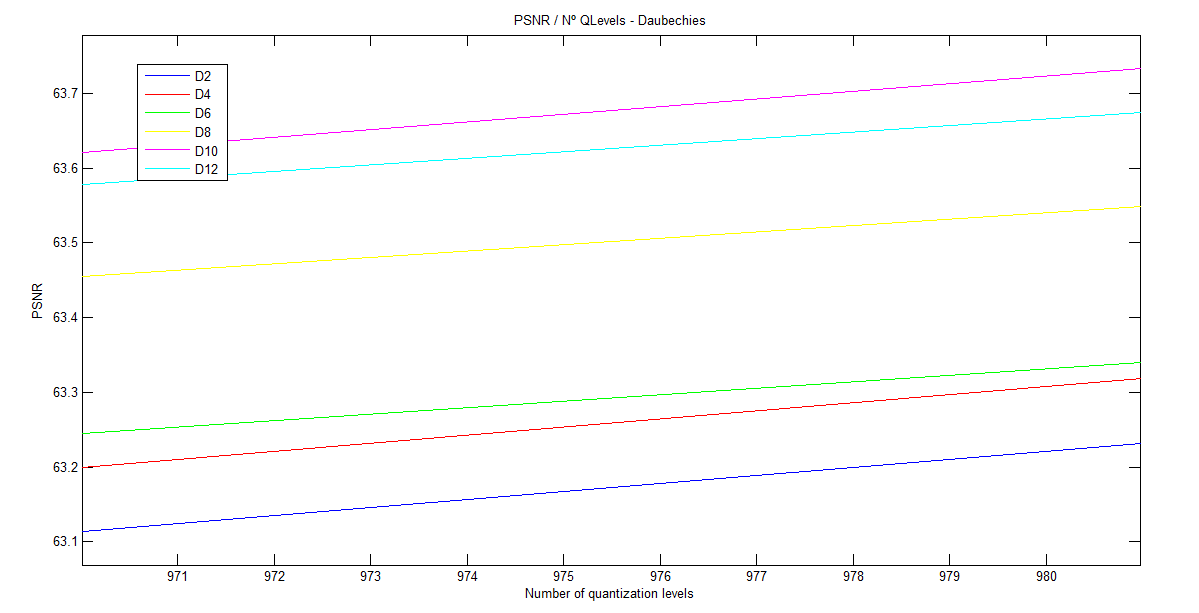
\includegraphics[scale=0.30]{reportImages/PSNR_Daubechies_detail1.PNG}
 		\caption{Detail 2 of PSNR}
 	\end{subfigure}
 	
 	\caption{Comparison for different number of quantization levels }
 	\label{Levels1}
 \end{figure}
 
 \subsection{Possible improvements for quantization}

For the quantization two great improvements could be performed.\\

First one is for the DCT, and the idea is to apply quantization only in the upper right quarter of the image, where the most of the data is saved. Most of the information will be processed and time and space will be reduced quantitatively. 

The quantization could be improved using an iterative algorithm that optimize the levels grouping the stretched distribution. This algorithm is called Lloyd's algorithm and will achieve the perfect distribution among the levels because the centroids and borders of them move after each iteration. It will take much longer time to converge if the tolerance is too low.


%The image in this example will be split into magnitude and phase, and it will be reconstructed later on from this two parts, allowing to show the inversibility of the Fourier transform in absence of noise. 
% \begin{figure}[H]
% 	\centering
% 	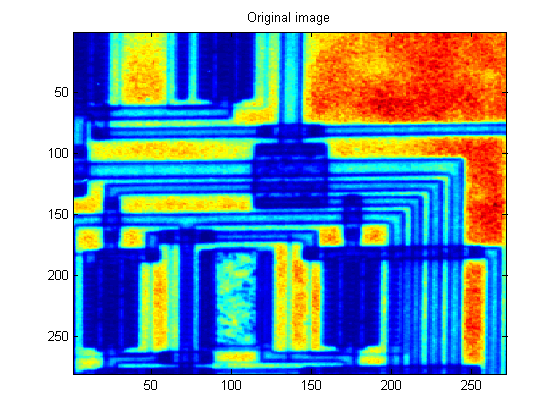
\includegraphics[width=0.5\textwidth]{reportImages/exp1_original.png} %
% 	\caption{Original image}
% 	\label{original}
% \end{figure} 
%The image could be seen in the color map to allow a better visualization. From the original image the magnitude and the phase could be obtained applying  the Fourier transform for each pixel. This transformation and the magnitude and phase images are calculated as follows.
%\begin{eqnarray}
%F(u,v)=\sum_{x=0}^{N}\sum_{y=0}^{M}f(x,y)\exp^{-2\pi j\left(\frac{xy}{M}+\frac{yv}{N}\right)}\\
%\left|F(u,v)\right|=\sqrt{Re^{2}\left(F(u,v)\right)+Im^{2}\left(F(u,v)\right)}\\
%\angle F(u,v) = \arctan\left(\frac{Im\left(F(u,v)\right)}{Re\left(F(u,v)\right)}\right)
%\end{eqnarray}
%Where \textit{$Im\left(F(u,v)\right)$} represents the imaginary part of the Fourier transform while \textit{$Re\left(F(u,v)\right)$} represents the real part.
%The results of getting each one of these images and the posterior reconstruction could be seen in Fig.\ref{exp1}
%\begin{figure}[H]
% 	\centering
% 	\begin{subfigure}{0.32\textwidth} 
% 		\centering						
% 		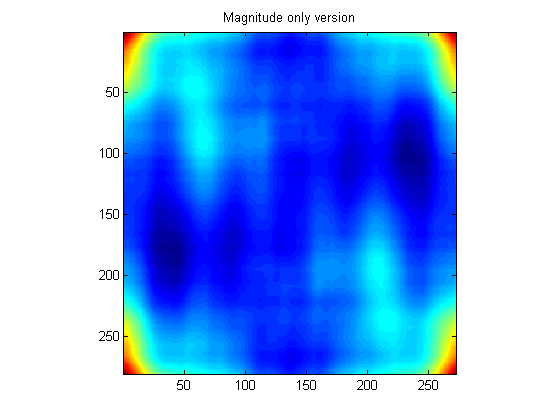
\includegraphics[scale=0.5]{reportImages/exp1_magnitude.PNG}
%		\caption{Magnitude of the Fourier transform image}
%	\end{subfigure}
%	\begin{subfigure}{0.32\textwidth}
%		\centering
%		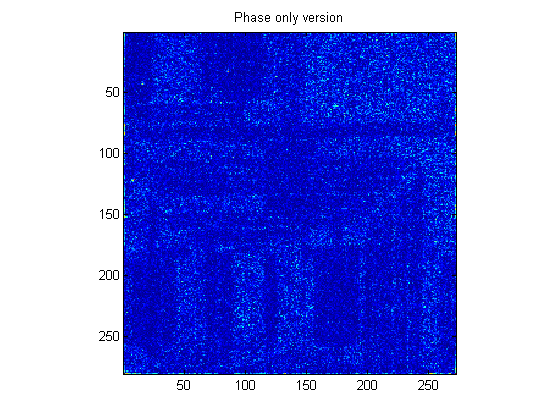
\includegraphics[scale=0.5]{reportImages/exp1_phase.PNG}
%		\caption{Phase of the Fourier transform image}
%	\end{subfigure}
%	\begin{subfigure}{0.32\textwidth}
%		\centering
%		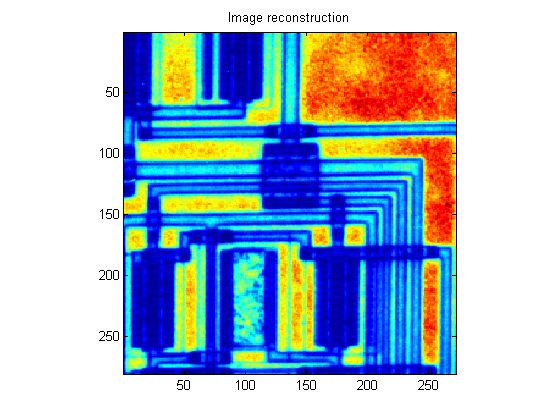
\includegraphics[scale=0.5]{reportImages/exp1_reconstructed.PNG}
%		\caption{Reconstructed image}
%	\end{subfigure}
%	\caption{Reconstruction of an image from its magnitude and phase}
%	\label{exp1}
%\end{figure}
%The magnitude is giving a measure of the how much is any frequency in the original image, while the phase is given the position of each of these frequencies in the image. For mathematical reasons the Fourier transform image is always symmetrical respect the origin, so is centered at this position and displayed in a logarithmic scale.\\
%
%In the next example the reconstruction of the image will try to be implemented after making a random phase for each of the pixels. In this way all the space information will be lost and the reconstruction will not be nearly close to the original image.
%\begin{figure}[H]
%	\centering
%	\begin{subfigure}{0.49\textwidth} 
%		\centering						
%		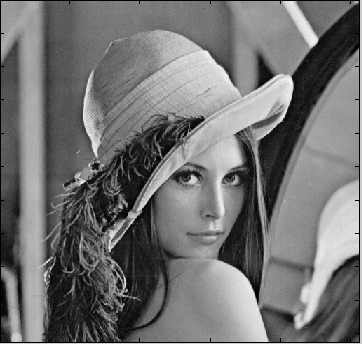
\includegraphics[scale=0.5]{reportImages/exp1_lena.PNG}
%		\caption{Original image: Lena}
%	\end{subfigure}
%	\begin{subfigure}{0.49\textwidth}
%		\centering
%		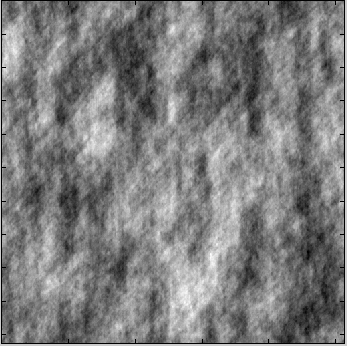
\includegraphics[scale=0.5]{reportImages/exp1_random_phase.PNG}
%		\caption{Reconstruction with a random phase}
%	\end{subfigure}
%	\label{exp1_1}
%\end{figure}
%If the same experiment is performed over an image with low space correlation, the reconstructed image will have a similar appearance. The gray levels should have the same number of pixels for both of the images.
%
%\begin{figure}[H]
%	\centering
%	\begin{subfigure}{0.49\textwidth} 
%		\centering						
%		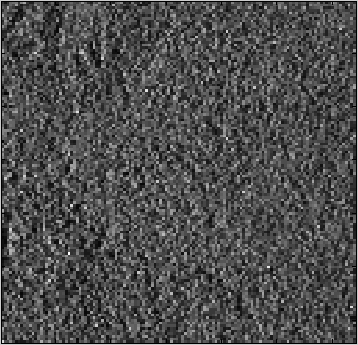
\includegraphics[scale=0.5]{reportImages/exp1_sar.PNG}
%		\caption{Original image: Sar}
%	\end{subfigure}
%	\begin{subfigure}{0.49\textwidth}
%		\centering
%		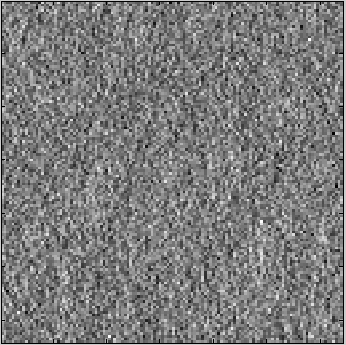
\includegraphics[scale=0.5]{reportImages/exp1_sar_random_phase.PNG}
%		\caption{Reconstruction with a random phase}
%	\end{subfigure}
%	\label{exp1_2}
%\end{figure}
%
%In the case that the magnitude were replaced by random values, the spatial information will remain, but not the intensities for each pixel. The reconstruction for the image could be seen in the next picture.
%
% \begin{figure}[H]
% 	\centering
% 	\begin{subfigure}{0.49\textwidth} 
% 		\centering						
% 		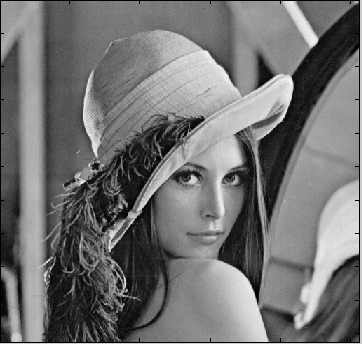
\includegraphics[scale=0.5]{reportImages/exp1_lena.PNG}
% 		\caption{Original image: Lena}
% 	\end{subfigure}
% 	\begin{subfigure}{0.49\textwidth}
% 		\centering
% 		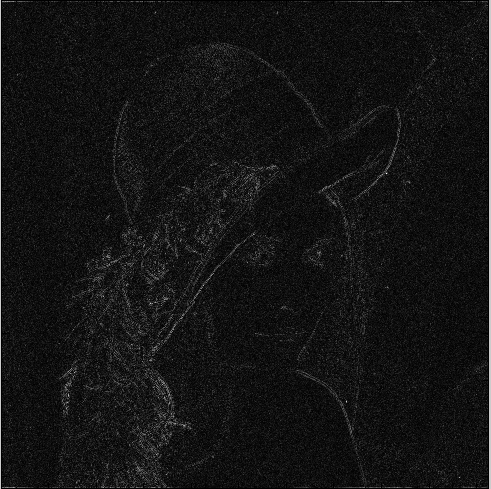
\includegraphics[scale=0.37]{reportImages/exp1_random_mag.PNG}
% 		\caption{Reconstruction with a random magnitude}
% 	\end{subfigure}
% 	\label{exp1_3}
% \end{figure}
% Repeating the experiment for \textit{'Sar.bmp'} is possible to appreciate that no special information is remaining.
% \begin{figure}[H]
% 	\centering
% 	\begin{subfigure}{0.49\textwidth} 
% 		\centering						
% 		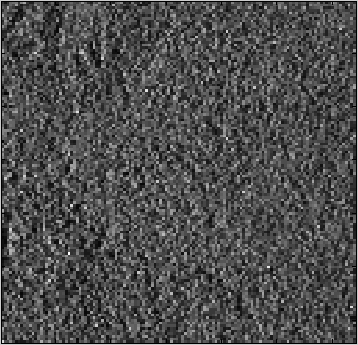
\includegraphics[scale=0.5]{reportImages/exp1_sar.PNG}
% 		\caption{Original image: Lena}
% 	\end{subfigure}
% 	\begin{subfigure}{0.49\textwidth}
% 		\centering
% 		
\includegraphics[scale=1]{reportImages/exp1_sar_random_mag.PNG}
% 		\caption{Reconstruction with a random magnitude}
% 	\end{subfigure}
% 	\label{exp1_4}
% \end{figure}
%
%\section{Fourier analysis and filtering}
%\subsection{Simple Fourier filtering}
%In this case it is going to be shown how is possible to perform a low-pass filtering by removing the higher frequencies from a certain image.
%
%\begin{figure}[H]
%	\centering
%	\begin{subfigure}{0.32\textwidth} 
%		\centering						
%		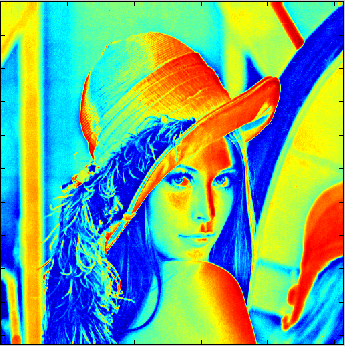
\includegraphics[scale=0.5]{reportImages/exp2_lena.PNG}
%		\caption{Original image}
%	\end{subfigure}
%	\begin{subfigure}{0.32\textwidth}
%		\centering
%		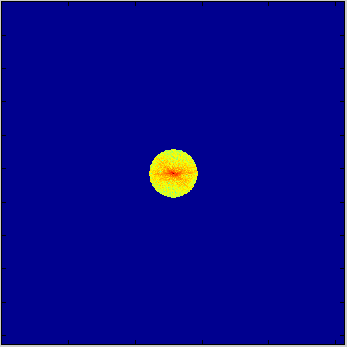
\includegraphics[scale=0.5]{reportImages/exp2_lena_filer_01.PNG}
%		\caption{Cutting off the high frequencies}
%	\end{subfigure}
%	\begin{subfigure}{0.32\textwidth}
%		\centering
%		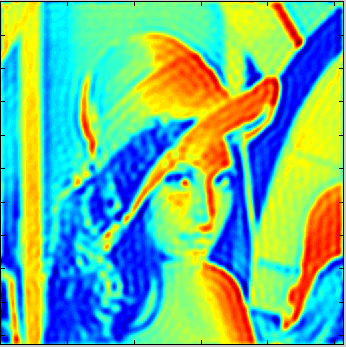
\includegraphics[scale=0.5]{reportImages/exp2_lena_filered_01.PNG}
%		\caption{Filtered image}
%	\end{subfigure}
%	\caption{Reconstruction of an image from its magnitude and phase}
%	\label{exp2_lowPass}
%\end{figure} 
% The problem with this kind of filtering is that the noise, that is in high frequencies, is being removed, but the edges are being removed as well. The use of removing certain frequencies using this filter is great when the noise has a known frequency, then a notch filter could be applied. 
% 
%\subsection{Developing FFT package}
% In this section  the code to compute the FFT will be developed. The following steps has been followed.
% \begin{enumerate}
% 	\item{Multiply the input image by (-1)x+y to center the transform for filtering}. It will allow to concentrate low frequencies in the center of the image
% 	\item{Compute the 2-D DFT and  the spectrum} Once in the frequency domain the filtering would be possible.
% 	\item{Multiply the resulting (complex) array by a real filter function (in the sense that the the real coefficients multiply both the real and imaginary parts of the transforms).} This is the way of choosing which frequencies will be cut and which ones will remain.
% 	\item{Compute the inverse 2-D Fourier transform.} Changing from the frequency domain to the space domain.
% 	\item{Multiply the result by (-1)x+y and take the real part} It is necessary to recover the original position of each pixel. 
% \end{enumerate}
% The original image, mask for the filter and result could be seen in Fig.\ref{exp2_FFT}
% \begin{figure}[H]
% 	\centering
% 	\begin{subfigure}{0.32\textwidth} 
% 		\centering						
% 		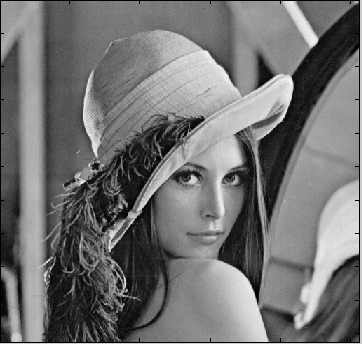
\includegraphics[scale=0.5]{reportImages/exp1_lena.PNG}
% 		\caption{Original image}
% 	\end{subfigure}
% 	\begin{subfigure}{0.32\textwidth}
% 		\centering
% 		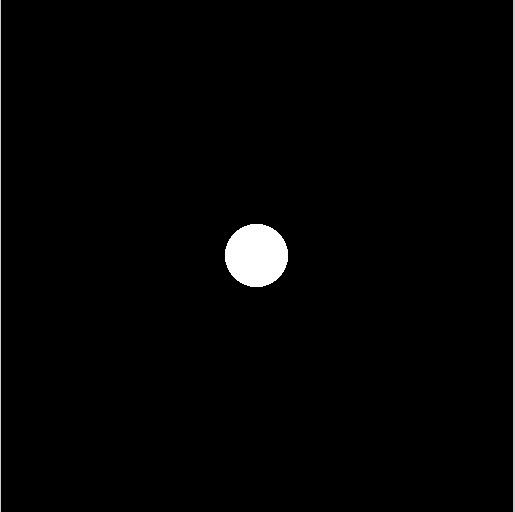
\includegraphics[scale=0.336]{reportImages/mask.PNG}
% 		\caption{Cutting off the high frequencies}
% 	\end{subfigure}
% 	\begin{subfigure}{0.32\textwidth}
% 		\centering
% 		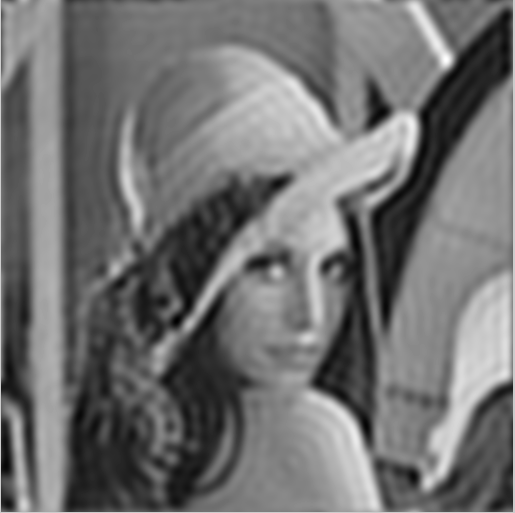
\includegraphics[scale=0.336]{reportImages/lena_FFT.PNG}
% 		\caption{Filtered image}
% 	\end{subfigure}
% 	\caption{Use of the FFT to filter an image}
% 	\label{exp2_FFT}
% \end{figure} 
% 
% \subsection{Fourier Spectrum and Average Value}
% There is a relationship between the maximum value in the Fourier domain and the average value of the image in the space domain. The maximum value (the center) in the Fourier domain divided by the total amount of pixels is the average value in the original image.
% \begin{figure}[H]
% 	\centering
% 	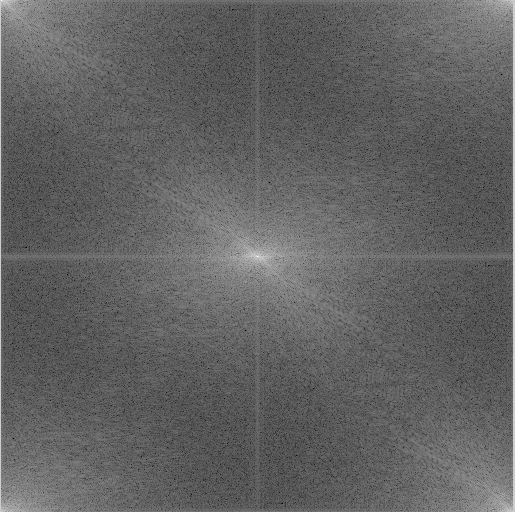
\includegraphics[width=0.3\textwidth]{reportImages/exp2_3_spectrum.png} %
% 	\caption{Spectrum of FFT for 'lena.png'}
% 	\label{Average}
% \end{figure}
% The average value in the original image is 124.0505, while the one obtained from the center of the spectrum is exactly the same .
% 
% \section{Compression and DCT}  
% Last experiment will consist in analyze how precision of the quantization in the spectrum will affect to the results of the image.
% First, let's check how the quality of the reconstructed image is affected when the original image of Lena is quantized in magnitude but not in phase. This will be achieved setting the maximum levels of quantization (512x512) for the phase to the total amount of pixels in the image and the levels of quantization for the phase as the closer integer to the 10\% of the number of pixels of the image.
%  \begin{figure}[H]
%  	\centering
%  	\begin{subfigure}{1\textwidth} 
%  		\centering						
%  		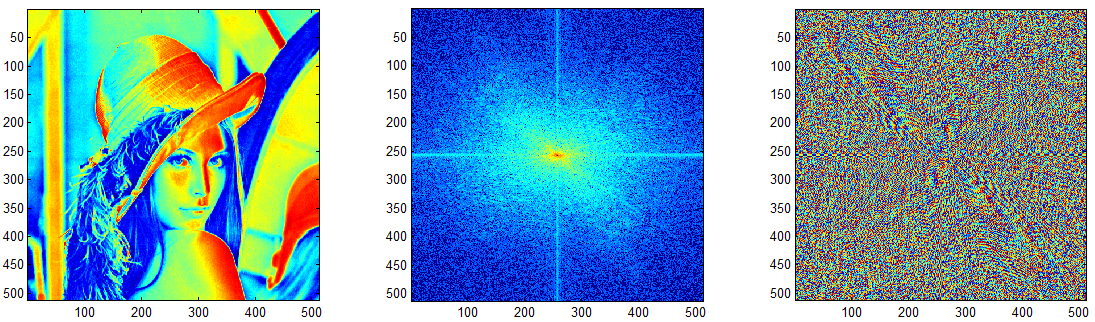
\includegraphics[scale=0.5]{reportImages/exp3_magnitude01.PNG}
%  		\caption{Original image, magnitude, and phase}
%  	\end{subfigure}
%  	\begin{subfigure}{1\textwidth}
%  		\centering
%  		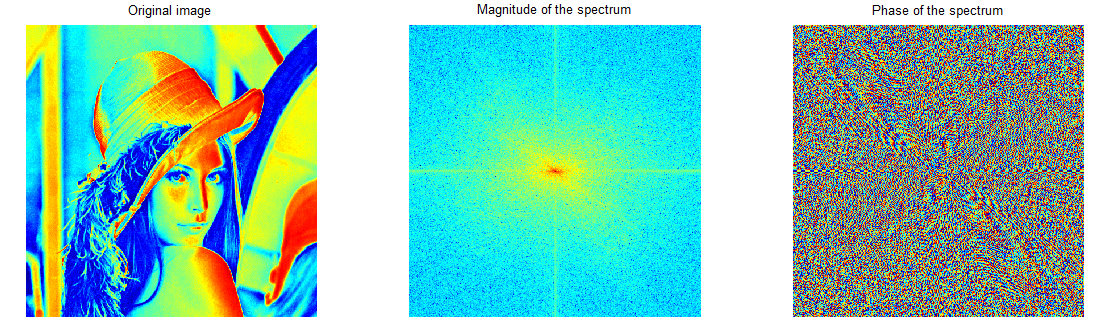
\includegraphics[scale=0.5]{reportImages/exp3_magnitude_compressed01.PNG}
%  		\caption{Quantized in magnitude and phase}
%  	\end{subfigure}
%  	\begin{subfigure}{0.32\textwidth}
%  		\centering
%  		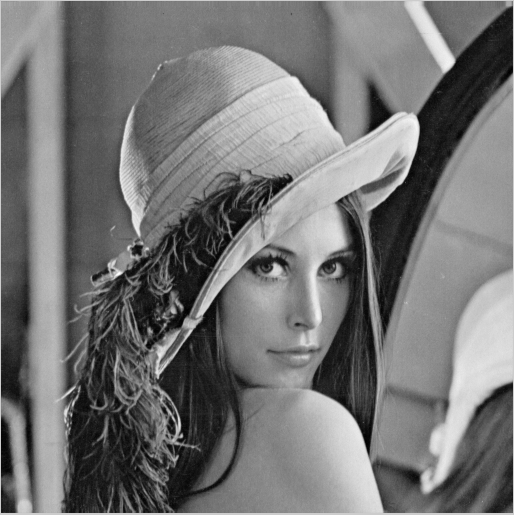
\includegraphics[scale=0.336]{reportImages/exp3_lena_magnitude_compressed01.PNG}
%  		\caption{Result of reconstruction}
%  	\end{subfigure}
%  	\caption{Quantization of the magnitude to 10\% of original size}
%  	\label{exp3_mag}
%  \end{figure}
%  
%  If  the process is repeated for different values of the quantization level for the magnitude the results are like in Fig.\ref{exp3_mag_1}
%  \begin{figure}[H]
%  	\centering
%  	\begin{subfigure}{0.32\textwidth} 
%  		\centering						
%  		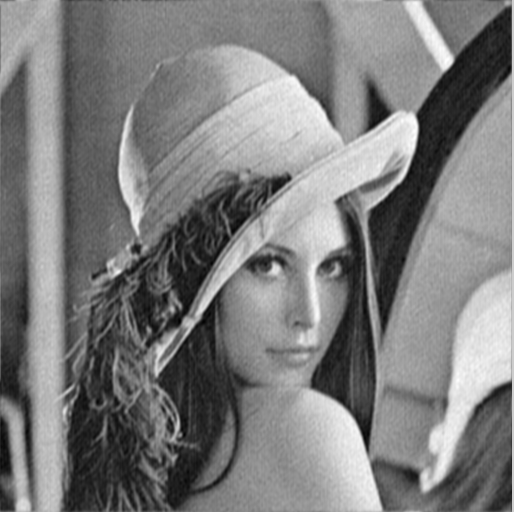
\includegraphics[scale=0.33]{reportImages/exp3_mag001.PNG}
%  		\caption{1\% of NxM = 2622}
%  	\end{subfigure}
%  	\begin{subfigure}{0.32\textwidth}
%  		\centering
%  		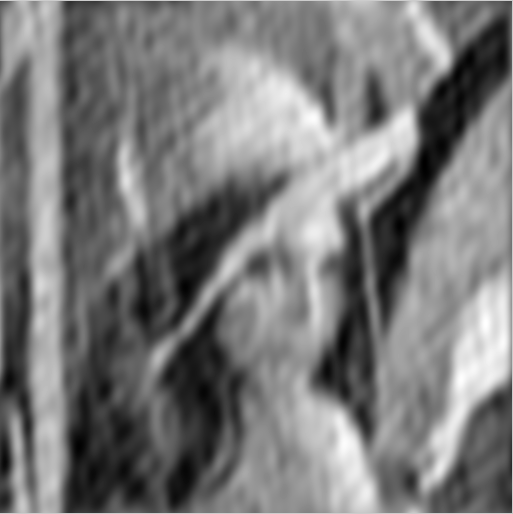
\includegraphics[scale=0.33]{reportImages/exp3_mag0001.PNG}
%  		\caption{0.1\% of NxM = 262}
%  	\end{subfigure}
%  	\begin{subfigure}{0.32\textwidth}
%  		\centering
%  		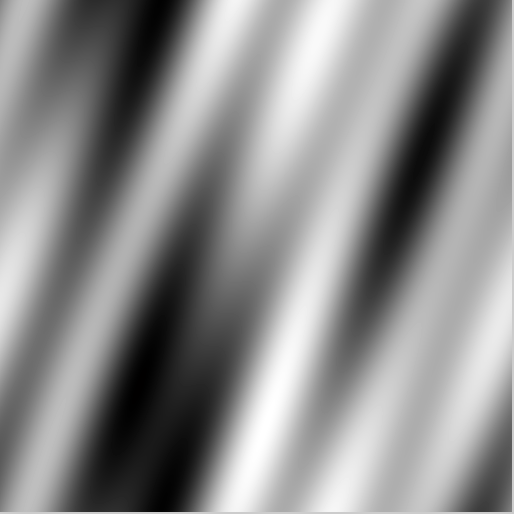
\includegraphics[scale=0.33]{reportImages/exp3_mag00001.PNG}
%  		\caption{0.01\% of NxM = 26}
%  	\end{subfigure}
%  	\caption{Varying the quantization levels for the magnitude}
%  	\label{exp3_mag_1}
%  \end{figure}
%   
%  In an analog way is possible to reduce the amount of levels for the quantization with respect to the phase. It will be shown that a lower amount of levels will be needed to recover the image with an acceptable quality.
%  \begin{figure}[H]
%  	\centering
%  	\begin{subfigure}{0.24\textwidth} 
%  		\centering						
%  		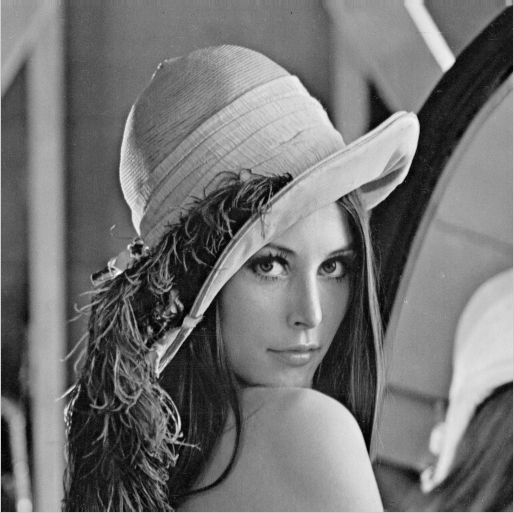
\includegraphics[scale=0.3]{reportImages/exp3_phase001.PNG}
%  		\caption{1\% of NxM = 2622}
%  	\end{subfigure}
%  	\begin{subfigure}{0.24\textwidth}
%  		\centering
%  		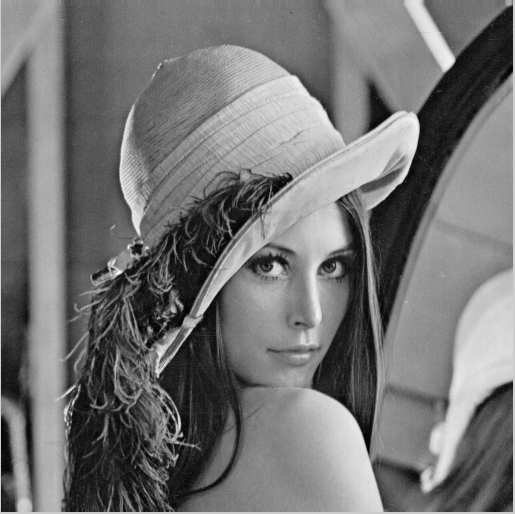
\includegraphics[scale=0.3]{reportImages/exp3_phase0001.PNG}
%  		\caption{0.1\% of NxM = 262}
%  	\end{subfigure}
%  	\begin{subfigure}{0.24\textwidth}
%  		\centering
%  		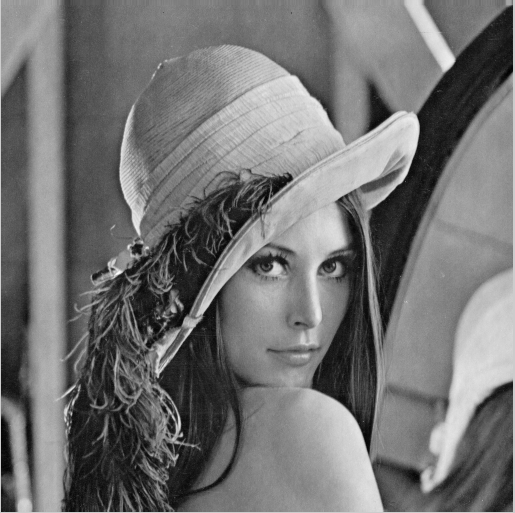
\includegraphics[scale=0.3]{reportImages/exp3_phase00001.PNG}
%  		\caption{0.01\% of NxM = 26}
%  	\end{subfigure}
%  	\begin{subfigure}{0.24\textwidth}
%  		\centering
%  		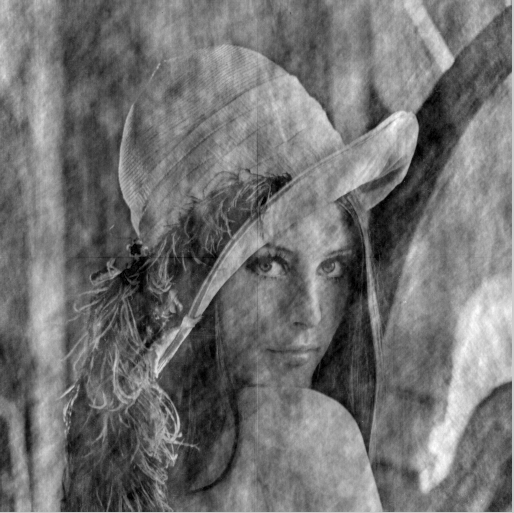
\includegraphics[scale=0.3]{reportImages/exp3_phase000001.PNG}
%  		\caption{0.001\% of NxM = 3}
%  	\end{subfigure}
%  	
%  	\caption{Varying the quantization levels for the magnitude}
%  	\label{exp3_phase_1}
%  \end{figure}
%%%  As a conclusion for this part is has to be said that is much suitable to quantize in a lower number of levels the phase than the magnitude. In the case of reducing the number of levels in the magnitude the edges will be progressively affected and as a consequence the image will become blurry. In the case of reducing the number of levels for the phase, the image would like degraded remaining the edges.
  
\begin{thebibliography}{99}
%%

\bibitem{c1}
'Advanced Image Analysis Notes', Mathini Sellathurai, Heriot Watt University, 2014
%%
%%\bibitem{c3}
%%'Ultrasound Image Enhancement Based on Image Compounding' - Yair Kerner - Technion (Israel Institute of Technology) - Haifa - June 2004 
%%
%%\bibitem{c4}
%%'Physical Principles of General and Vascular Sonography' - Jim Baun - San Francisco, CA -March 2009
%%
%%\bibitem{c5}
%%'Physical Principles of General and Vascular Sonography' - Jim Baun - San Francisco, CA -March 2009
%%
%%\bibitem{c6}
%%'Image Formation and Image Processing in Ultrasound' - Jeffrey C. Bamber - Institute of Cancer Research and The Royal Marsden NHS Trust, Surrey, SM2 5PT
\end{thebibliography}

\end{document}
